%# -*- coding: utf-8-unix -*-
% !TEX program = xelatex
% !TEX root = ../thesis.tex
% !TEX encoding = UTF-8 Unicode
\chapter{系统设计}
完成系统的定义阶段之后,便进入了系统的设计阶段,
主要完成对系统的结构设计、系统模块设计与数据库表结构设计。
\section{系统框架结构设计}
本系统为满足不依赖网络、随时可用和安全性的特点,采用单用户体系结构,
但在此基础上预留了系统接口,保证后续的可拓展性。

\begin{figure}[H]
	\centering
	\makebox[\textwidth]{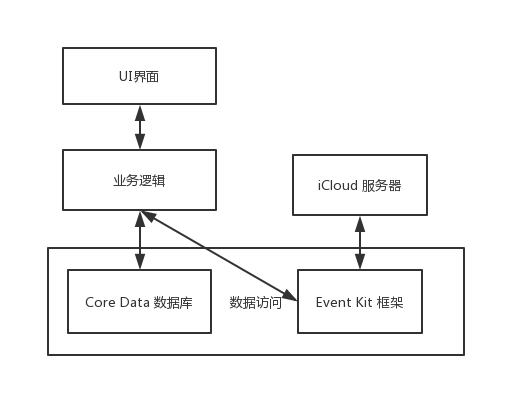
\includegraphics[height=8cm]{figure/level.png}}
	\caption{系统框架结构示意图}
    \label{fig:level}
\end{figure}

Core Data 是Apple提供的持久化数据的方案,一般来说,底层使用的是 Sqlite 数据库,如下图所示。
\begin{figure}[H]
	\centering
	\makebox[\textwidth]{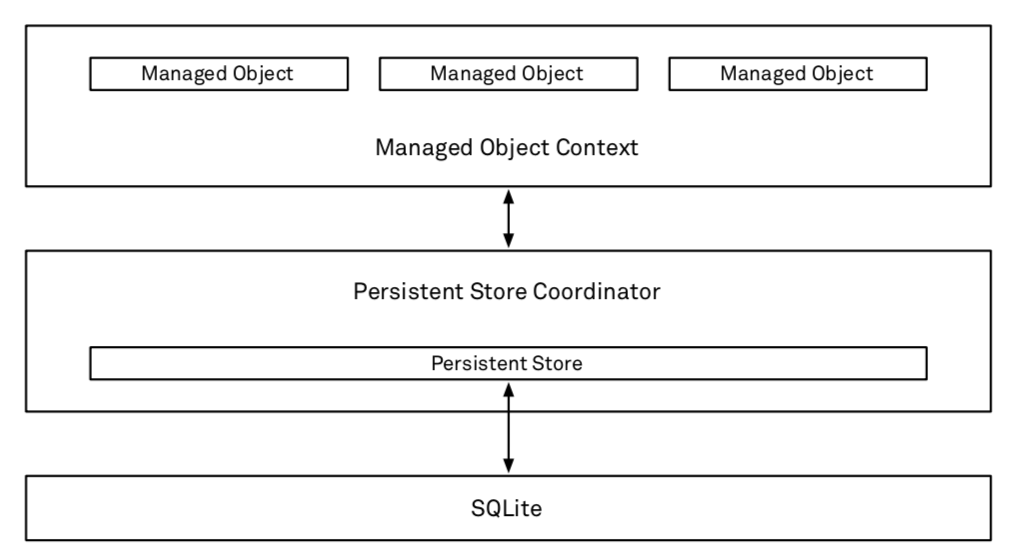
\includegraphics[height=6cm]{figure/core_data.png}}
	\caption{Core Data 结构示意图}
    \label{fig:core_data}
\end{figure}

\section{系统模块设计}
为保证系统的可拓展性和开发的便利,将系统分解为几个主要模块,如下图。
\begin{figure}[H]
	\centering
	\makebox[\textwidth]{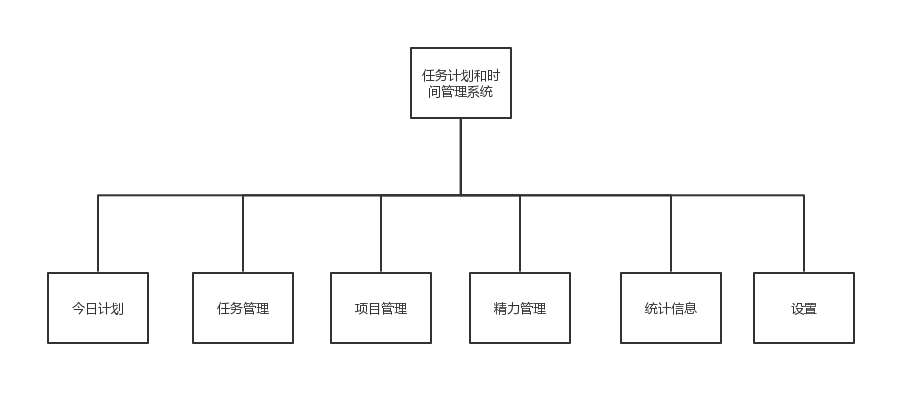
\includegraphics[width=\textwidth]{figure/part.png}}
	\caption{系统模块结构图}
    \label{fig:part}
\end{figure}

从图中可以看出任务计划及时间管理系统的架构设计,可以分为六个模块,
今日计划模块、任务管理模块、项目管理模块、精力管理模块、统计信息模块、设置模块,
系统通过用户输入获取信息,将信息保存到本地的数据库或系统的EventKit中,
再通过业务逻辑将信息经过排序、筛选等处理后进行展示。
其中每个模块均可直接通过主界面到达,将系统拆分为各个模块后,
降低了系统的耦合性,增强了系统的可拓展性。

\section{数据库设计}

\subsection{系统实体关系图}
\begin{figure}[H]
	\centering
	\makebox[\textwidth]{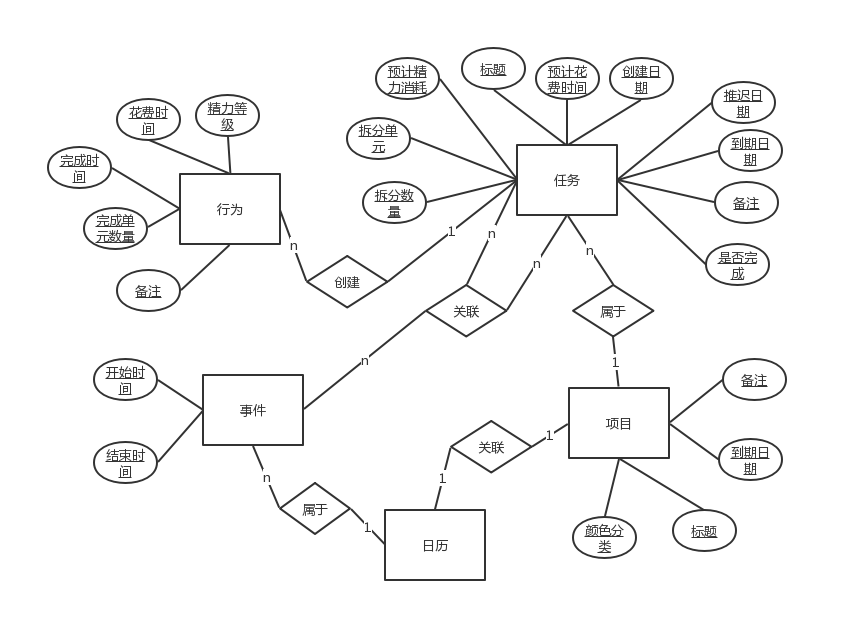
\includegraphics[width=\textwidth]{figure/e-r.png}}
	\caption{实体关系图}
    \label{fig:e-r}
\end{figure}


\subsection{系统数据表}
由于Core Data会通过数据表之间的概念数据模型和他们之间的关系生成相应的物理模型(包括ID和主外建等),
无需开发者生成具体的物理模型。
图\ref{fig:e-r}中出现的事件和日历均为iOS系统自带的实体,也无需保存入Core Data 数据库中。

\begin{figure}[H]
	\centering
	\makebox[\textwidth]{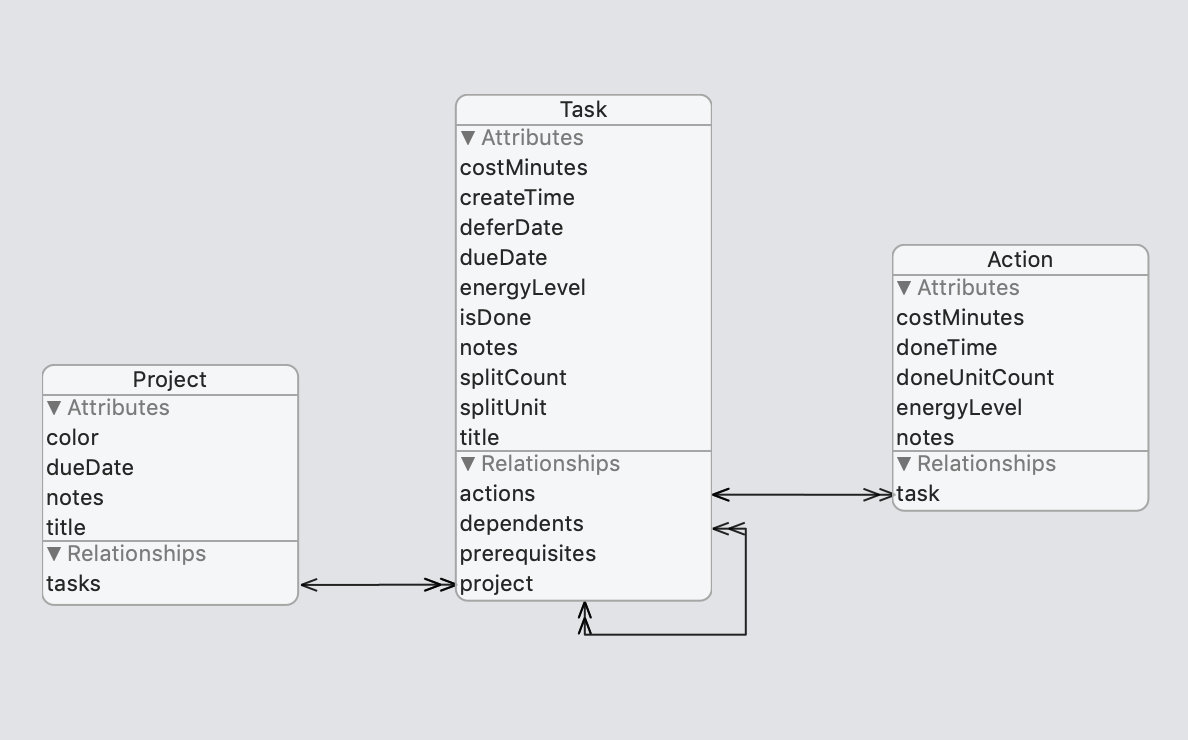
\includegraphics[width=\textwidth]{figure/relationship.png}}
	\caption{Core Data 数据实体及关系图}
\end{figure}

\begin{table}[H]
  \centering
  \caption{任务表}
  \begin{tabular}{ccccccc} \toprule
	序号 & 列名 & 数据类型 & 允许空 & 说明 & 备注 \\
	\midrule
	1 & costMinutes & Integer32 & 否 & 花费时间 & 无 \\
	2 & createTime & Date & 否 & 创建时间 & 无 \\
	3 & deferDate & Date & 否 & 推迟日期 & 无 \\
	4 & dueDate & Date & 否 & 到期时间 & 无 \\
	5 & energyLevel & Integer16 & 否 & 精力等级 & 无 \\
	6 & isDone & Boolean & 否 & 是否完成 & 无 \\
	7 & notes & String & 否 & 备注 & 无 \\
	8 & splitCount & Integer32 & 否 & 拆分数量 & 无 \\
	9 & splitUnit & String & 否 & 拆分单位 & 无 \\
	10 & title & String & 否 & 标题 & 无 \\
	\bottomrule
  \end{tabular}
\end{table}

\begin{table}[H]
	\centering
	\caption{项目表}
	\begin{tabular}{ccccccc} \toprule
	  序号 & 列名 & 数据类型 & 允许空 & 说明 & 备注 \\
	  \midrule
	  1 & color & Transformable & 否 & 花费时间 & UIColor \\
	  2 & dueDate & Date & 否 & 到期时间 & 无 \\
	  3 & notes & String & 否 & 备注 & 无 \\
	  4 & title & String & 否 & 题目 & 无 \\
	  \bottomrule
	\end{tabular}
\end{table}

\begin{table}[H]
	\centering
	\caption{行为表}
	\begin{tabular}{ccccccc} \toprule
	  序号 & 列名 & 数据类型 & 允许空 & 说明 & 备注 \\
	  \midrule
	  1 & costMinutes & Integer32 & 否 & 花费时间 & UIColor \\
	  2 & doneTime & Date & 否 & 完成时间 & 无 \\
	  3 & doneUnitCount & Integer32 & 否 & 完成数量 & 无 \\
	  4 & energyLevel & Integer16 & 否 & 精力花费 & 无 \\
	  5 & notes & String & 否 & 备注 & 无 \\
	  \bottomrule
	\end{tabular}
\end{table}

